\let\negmedspace\undefined
\let\negthickspace\undefined
\documentclass[journal,12pt,onecolumn]{IEEEtran}
\usepackage{cite}
\usepackage{amsmath,amssymb,amsfonts,amsthm}
\usepackage{algorithmic}
\usepackage{graphicx}
\usepackage{textcomp}
\usepackage{xcolor}
\usepackage{txfonts}
\usepackage{listings}
\usepackage{enumitem}
\usepackage{mathtools}
\usepackage{gensymb}
\usepackage{comment}
\usepackage[breaklinks=true]{hyperref}
\usepackage{tkz-euclide} 
\usepackage{gvv}                                        
%\def\inputGnumericTable{}                                 
\usepackage[latin1]{inputenc}     
\usepackage{xparse}
\usepackage{color}                                            
\usepackage{array}                                            
\usepackage{longtable}                                       
\usepackage{calc}                                             
\usepackage{multirow}
\usepackage{multicol}
\usepackage{hhline}                                           
\usepackage{ifthen}                                           
\usepackage{lscape}
\usepackage{tabularx}
\usepackage{float}
\newtheorem{theorem}{Theorem}[section]
\newtheorem{problem}{Problem}
\newtheorem{proposition}{Proposition}[section]
\newtheorem{lemma}{Lemma}[section]
\newtheorem{corollary}[theorem]{Corollary}
\newtheorem{example}{Example}[section]
\newtheorem{definition}[problem]{Definition}
\newcommand{\BEQA}{\begin{eqnarray}}
\newcommand{\EEQA}{\end{eqnarray}}
\newcommand{\define}{\stackrel{\triangle}{=}}
\theoremstyle{remark}
\newtheorem{rem}{Remark}
% Marks the beginning of the document
\begin{document}
\title{PI : PRODUCTION AND INDUSTRIAL ENGINEERING}
\author{AI25BTECH11034 - Sujal Chauhan}
\maketitle
\renewcommand{\thefigure}{\theenumi}
\renewcommand{\thetable}{\theenumi}
\textbf{Q.1-Q.20 carry one marks each}
\vspace{1cm}

\begin{enumerate}

    

    \item %Q.1}]  
    The value of the integral $\int_{-\frac{\pi}{2}}^{\frac{\pi}{2}}xcos(x)dx$ is 
    \hfill{(PI 2008)}
    \begin{multicols}{4}
    \begin{enumerate}
        \item $0$
        \item $\pi-2$
        \item $\pi$
        \item $\pi+2$
    \end{enumerate}
\end{multicols}
\vspace{1cm}
\item %Q.2}] 
The value of the expression $$\frac{-5+i10}{3+i4}$$ is 
    \hfill{(PI 2008)}
    \begin{multicols}{4}
    \begin{enumerate}
        \item $1-i2$
        \item $1+i2$
        \item $2-i$
        \item $2+i$
    \end{enumerate}
\end{multicols}
\vspace{1cm}
\item %Q.3}] 
The value of the expression $$\lim_{x\to0}\left[\frac{\sin(x)}{e^xx}\right]$$  
    \hfill{(PI 2008)}
    \begin{multicols}{4}
    \begin{enumerate}
        \item $0$
        \item $\frac{1}{2}$
        \item $1$
        \item $\frac{1}{1+e}$
    \end{enumerate}
\end{multicols}
\vspace{1cm}
\item %Q.4}]
In inventory cost structure, set up cost is a part of  replenishment cost when it
    \hfill{(PI 2008)}
    \begin{itemize}[label={}]
        \item a has taken place externally
        \item b) is dependent on supply conditions
        \item c) is independent of supply conditions
        \item d) has taken place internally
    \end{itemize}
    \vspace{1cm}
    \item %Q.5}]
    Acceptable Quantity Level(AQL) is associated with
    \hfill{(PI 2008)}

\begin{itemize}
        \item a Producer's risk
        \item b) Consumer's risk
        \item c) Lot tolerance percent defective
        \item d) Average outgoing quality limit
    \end{itemize}
\vspace{1cm}
\item %Q.6}] 
The REL chart is used for 
    \hfill{(PI 2008)}

\begin{itemize}
        \item a designing the layout of plants
        \item b) estimating the valuation of stock
        \item c) analysing the movement of an item in a store
        \item d) maintaining the issue and reciept record
    \end{itemize}
    \vspace{1cm}
    \item %Q.7}]  
    If $\Vec{r}$ is the position vector of any point on a closed surface $S$ that encloses the volume $V$, then    
    $\int_{S}\left(\vec{r}.d\vec{S}\right)$ 
    \hfill{(PI 2008)}
    \begin{multicols}{4}
    \begin{enumerate}
        \item $\frac{1}{2}V$
        \item $V$
        \item $2V$
        \item $3V$
    \end{enumerate}
\end{multicols}
\vspace{1cm}
\item %Q.8}] 
Laplace transform of $8t^3$ is     \hfill{(PI 2008)}
    \begin{multicols}{4}
    \begin{enumerate}
        \item $\frac{8}{s^4}$
        \item $\frac{16}{s^4}$
        \item $\frac{24}{s^4}$
        \item $\frac{48}{s^4}$
    \end{enumerate}
\end{multicols}
\vspace{1cm}
\item  %Q.9}] 
For a random variable $x (-\infty<x<\infty)$ following normal distribution, the mean is $\mu=100$. If the probability is $P=\alpha$ for $x\geq110$, then the probability of $x$ lying between 90 and 110,i.e.,$P(90\leq x \leq 110 )$ will be equal to
    \hfill{(PI 2008)}
    \begin{multicols}{4}
    \begin{enumerate}
        \item $1-2\alpha$
        \item $1-\alpha$
        \item $1-\frac{\alpha}{2}$
        \item $2\alpha$
    \end{enumerate}
\end{multicols}
\vspace{1cm}
\item %Q.10}]
Consider a steady,reversible flow process in a system with one inlet stream and one outlet stream. Potential and kinetic energy effects are negligibly small. Given : $\nu=$specific volume and $p=$pressure of the system. The net work done by system per unit mass flow rate is 
    \hfill{(PI 2008)}
    \begin{multicols}{4}
    \begin{enumerate}
        \item $\int pdv$
        \item $-\int pdv$
        \item $\int vdp$
        \item $-\int vdp$
    \end{enumerate}
\end{multicols}
\vspace{1cm}
\item %Q.11}]
A refrigerator,operating in a room at a temprature of $29.5^{\circ}C$, maintains the refrigerated space at $2^{\circ}C$. The maximum possible COP of the refrigerator is 
    \hfill{(PI 2008)}
    \begin{multicols}{4}
    \begin{enumerate}
        \item $1.0$
        \item $7.0$
        \item $10.0$
        \item $11.0$
    \end{enumerate}
\end{multicols}
\vspace{1cm}
\item %Q.12}]
Self locking condition for a pair of square thread screw and nut having coeffficent of friction$\mu=$, lead of thread$=L$ and pitch diameter of thread $=d$, is given by
    \hfill{(PI 2008)}
    \begin{multicols}{4}
    \begin{enumerate}
        \item $d>\frac{L}{\pi\mu}$
        \item $d>\pi\mu L$
        \item $d>\mu L$
        \item $\mu>Ld$
    \end{enumerate}
\end{multicols}
\vspace{1cm}
\item %Q.13}] 
The state of stress at a point in a body under plane state of stress condition is given by\[ \myvec {
60 && 0 \\
0 && 20
}\]
    \hfill{(PI 2008)}
    \begin{multicols}{4}
    \begin{enumerate}
        \item $0$
        \item $20$
        \item $30$
        \item $40$
    \end{enumerate}
\end{multicols}
\vspace{1cm}
\item %Q.14}] 
Which one of the following is a heat treatment process for surface hardening?
    \hfill{(PI 2008)}
    \begin{multicols}{4}
    \begin{enumerate}
        \item Normalizing
        \item Annneling
        \item Carburising
        \item Tempering
    \end{enumerate}
\end{multicols}
\vspace{1cm}
\item  %Q.15}] 
Which pair among the following solid waste welding process uses heat from a extrenal source?\\
P-Diffusion welding;Q-Friction welding;R-Ultrasonic welding;S-Forge welding
    \hfill{(PI 2008)}
    \begin{multicols}{4}
    \begin{enumerate}
        \item P and R
        \item R and S
        \item Q and S
        \item P and S
    \end{enumerate}
\end{multicols}
\vspace{1cm}
\item  %Q.16}]
In hollow cylindrical parts,made by centrifugal casting, the density of the part is 
    \hfill{(PI 2008)}
   \begin{itemize}[label={}]
        \item a) maximum at outer region
        \item b) maximum at inner region
        \item c) maximum at the mid-point between outer and inner surfaces
        \item d) uniform throught
    \end{itemize}
\vspace{1cm}

\item %Q.17}] 
Brittle material are machined with tools having zero or negative rake angle because it  
    \hfill{(PI 2008)}

\begin{itemize}[label={}]
        \item a) results in lower cutting force  
        \item b) improve surface finish
        \item c) provides adequate strenght to cutting tool
        \item d) results in more accurate dimensions 
    \end{itemize}
\vspace{1cm}

\item %Q.18}]
When 0.8\% carbon eutectoid steel is slowly cooled from $750^{\circ}$ to room temorature,
    \hfill{(PI 2008)}

\begin{itemize}[label={}]
        \item a) austenite transforms to pearlite
        \item b) pearlite transforms to austenite
        \item c) austenite transforms to martensite  
        \item d) pearlite transforms to martensite
    \end{itemize}
\vspace{1cm}
\item %Q.19}]
Which one of the following is a unary operation performed in relational data model?
    \hfill{(PI 2008)}

\begin{itemize}[label={}]
        \item aCartesian product            \item b)Set union 
        \item c)Set diffrence                \item d)Selection 
    \end{itemize}
\vspace{1cm}
\item %Q.20}]
The process of tracing through the MRP records and all levels in the product structure to identify how changes in the records of one component will effect the records of other components is known as
    \hfill{(PI 2008)}\\
    \begin{itemize}
        \item a product exlosion
        \item b) lead time offsetting
        \item c) updating
        \item d) pegging
    \end{itemize}
\vspace{1cm}
\textbf{Q.21-Q.75 carry two marks each}
\vspace{1cm}
\item %Q.21}]
The eigenvector pair of the matrix
\myvec 
{3 & 4 \\
4 & -3}
 is
    \hfill{(PI 2008)}\\
    \[\begin{matrix}
   { a \myvec { 2 \\ 1
    }  and \myvec { 1 \\-2
    }} & {b) \myvec { 2 \\ 1
    } and \myvec { 1 \\-2
    }}\\
    { c) \myvec { 2 \\ 1
    }  and \myvec { 1 \\-2
    }} & {d) \myvec { 2 \\ 1
    } and \myvec { 1 \\-2
    }}
    
    \end{matrix}\]
    \vspace{1cm}
    \item %Q.22}] 
    If the interval of integration is divided into two equal intervals of width 1.0, the value of the definite integral $\int_1^3 log_e x dx$, using Simpson's one-third rule, will be
    \hfill{(PI 2008)}
    \begin{multicols}{4}
    \begin{enumerate}
        \item $0.50$
        \item $0.80$
        \item $1.00$
        \item $1.29$
    \end{enumerate}
\end{multicols}
\item %Q.23}]
In a game,two players X and Y toss a coin alternately. Whosoever gets a 'head' first, wins the game and game is terminated. Assuming  that player X starts the game, the probability of player X winning is 
    \hfill{(PI 2008)}
    \begin{multicols}{4}
    \begin{enumerate}
        \item $\frac{1}{3}$
        \item $\frac{1}{2}$
        \item $\frac{2}{3}$
        \item $\frac{3}{4}$
    \end{enumerate}
\end{multicols}
\item %Q.24}]
Laplace transform of $\sinh (t)$ is  
    \hfill{(PI 2008)}
    \begin{multicols}{4}
    \begin{enumerate}
        \item $\frac{1}{s^2 -1}$
        \item $\frac{1}{1-s^2}$
        \item $\frac{s}{s^2-1}$
        \item $\frac{s}{1-s^2}$
    \end{enumerate}
\end{multicols}
\item %Q.25}]
A resorvoir contains an estimated 30,00,000 barrel of oil. The initial cost of the reservoir is Rs. 1,50,00,000. If 2,00,000 barrrels of oil are produced from the resorvoir during a particular year, how much will be the deplition charge (cost depletion) for that year?  
    \hfill{(PI 2008)}
    \begin{multicols}{4}
    \begin{enumerate}
        \item $Rs.10,00,000$
        \item $Rs.15,00,000$
        \item $Rs.20,00,000$
        \item $Rs.25,00,000$
    \end{enumerate}
\end{multicols}
\item %Q.26}] 
Customer arrives at a service counter nammed by a single person according to a Poisson distribution with a mean arrival rate of 30per hour. The time required to serve a customer follow and exponential distribuation with a mean of 100 seconds. The average waiting time (in hour) of a customer in the system will be
    \hfill{(PI 2008)}
    \begin{multicols}{4}
    \begin{enumerate}
        \item $0.138$
        \item $0.166$
        \item $0.276$
        \item $0.332$
    \end{enumerate}
\end{multicols}
\item %Q.27}]
Consider the following linear programming problem (LPP)  \\ \\
Maximize $z=5x_1+3x_2$\\
Subject to the following constraints
$x_1-x_2\leq2$\\
$x_1+x_2\geq 3$\\
$x_1,x_2\geq 0$
    \hfill{(PI 2008)}
    \begin{itemize}[label={}]
        \item a no solution
        \item b) unique solution
        \item c) two solution
        \item d) unbounded solution
    \end{itemize}
\vspace{1cm}
 \item %Q.28}]
 A machine costing Rs.2 lakh (salvage value of the machine at end of 4 years $= 0$) is to be depreciated over 4 years using the double declining balance depreciation method. The amount of depresiation changes in $3^{rd}$ year is 
    \hfill{(PI 2008)}
    \begin{multicols}{4}
    \begin{enumerate}
        \item Rs. $1.00$ lakh
        \item Rs. $0.50$ lakh
        \item Rs. $0.25$ lakh
        \item Rs. $0.125$ lakh
    \end{enumerate}
\end{multicols}
\vspace{1cm}
 \item %Q.29}]
 During a survey of customers in a store,20 samples of size 200 customers were taken. The number of dissatisfied customers was found to be 180. The upper and lower control limits for the control chart of disstisfied customers will be 
    \hfill{(PI 2008)}\\
\[ \begin{matrix}
       { a 18.345,0.205} & { a) 17.345,0.605} \\
       { a) 17.345,0.805} & { a) 16.345,0.705}
    \end{matrix}  \]
   
\vspace{1cm}

 \item %Q.30}] 
 An assembly has 10 components in series. Each component has an exponential time-to-failure distribution with a constant failure rare of 0.02 per 3000 hours of operation. Assuming that the failed component of the assembly is replaced immediately with another component that has the same failure rate, the relibility of the assmebly for 2000 hours of operation and the mean time-to-failure(MTTF) is 
    \hfill{(PI 2008)}
    \[
    \begin{matrix}
        {a) 0.875,10,000 hours } & {b)0.675,20,000 hours}\\
        {c)0.975,40,000 hours}  & {d)0.875,15,000 hours}
    \end{matrix}
    \]
    \vspace{1cm}
    \item %Q.31}]
    Match the following: 
    \hfill{(PI 2008)}\\
    \vspace{1cm}
    \begin{tabular}{p{4cm} p{6cm}}
\textbf{Group 1} & \textbf{Group 2} \\
    P--SLP                  & 1--Intellectual property system \\
    Q--Margin of Safety     & 2--Assembly line balancing\\
    R--LOB                  & 3--Facility design\\
    S--TRIPS                & Break even analysis\\
    \end{tabular}
    \vspace{1cm}
     \item %Q.32}]
     A man has deposited Rs. 1,000 per year for three year in bank that paid him 5\% intrest compounded annually. At the end three years,he had Rs 3,153 in his account. How much more would he have earned if the bannk had paid him 5\% intrest compounded continuously?
    \hfill{(PI 2008)}
    \begin{multicols}{4}
    \begin{enumerate}
        \item $Rs.300$
        \item $Rs30$
        \item $Rs3$
        \item $Rs0.30$
    \end{enumerate}
\end{multicols}
\vspace{1cm}

    \item %Q.33}] 
    Two pipes of uniform section but differnt diameter carry  water at the same volumetric flow rate. Water properties are the same in the two pipes. The Reynolds number,based on the pipe diameter.
    \hfill{(PI 2008)}
    \[
    \begin{matrix}
        {a) \text{is the same in both pipes}  } & {b)\text{is larger in the narrower pipe}}\\
        {c)\text{is smaller in the narrower pipe}}  & {d)\text{depends on the pipe material}}
    \end{matrix}
    \]
    \vspace{1cm}
     \item %Q.34}] 
     A single cylinder compression ignition engine, operating on the air-standard diesel cycle,has a mean effective pressure of 1.0MPa and a compression ratio of 21. The engine has a clearence volume of $5\times10^{-5}m^3$. The heat added at constant pressure is 2.0KJ. The thermal effciency of the engine is 
    \hfill{(PI 2008)}
    \begin{multicols}{4}
    \begin{enumerate}
        \item $10\%$
        \item $35\%$
        \item $50\%$
        \item $70\%$
    \end{enumerate}
\end{multicols}
\vspace{1cm}
 \item %Q.35}]
 An industrial gas $(C_p=1 KJ/kgK)$enters a parallel-flow heat exchanger at $250^{\circ}C$ with a flow rate of $2Kg/s$. The heat a water stream. Thenwater stream $(C_p=4KJ/kgK)$ enters the heat exchanger at  $50^{\circ}$ with a flow rate of $1kg/s$. The heat exchanger has an effectiveness of 0.75. The gas stream exit temprature will be 

    \hfill{(PI 2008)}
    \begin{multicols}{4}
    \begin{enumerate}
        \item  $75^{\circ}$
        \item  $100^{\circ}$

        \item  $125^{\circ}$

        \item  $150^{\circ}$

    \end{enumerate}
\end{multicols}
\vspace{1cm}
 \item %Q.36}]
 Oil is being pumped through a straight pipe. The pipe lenght, diameter and volumetric flow rate are all doubled in a new arrangment. The pipe friction factor, however, remains constant. The ratio of pipe frictional loses in the new arrangment to that in the original configuration would be   
    \hfill{(PI 2008)}
    \begin{multicols}{4}
    \begin{enumerate}
        \item $\frac{1}{4}$
        \item $\frac{1}{2}$
        \item $2$
        \item $4$
    \end{enumerate}
\end{multicols}
\vspace{1cm}
 \item %Q.37}]
 Air flows steadily at low speed throught a horizontal nozzle, which dischrages the air into the atmosphere. The area at the nozzle inlet and outlet are $0.1m^2$ and $0.2m^2$ respectively. If the air density remains constant at $1.0kg/m^3$, the gauge pressure(in kPa) required at the nozzle inlet to produce an outlet speed of 50 m/s would be  
    \hfill{(PI 2008)}
    \begin{multicols}{4}
    \begin{enumerate}
        \item $0.6$
        \item $1.2$
        \item $100.2$
        \item $101.2$
    \end{enumerate}
\end{multicols}
\vspace{1cm}
 \item %Q.38}]
 Heat is being transferred convextively from a cylindrical nuclear reactor fuel rod of 50 mm diameter to water at $75^{\circ}C$, Under steady state condition, the rate of heat genration within the fuel element is $5\times10^7W/m^3$ and the convection heat transfer coefficient is $1kW/m^2K$. \\
 The outer surface surface temprature of the fuel element would be
    \hfill{(PI 2008)}
    \begin{multicols}{4}
    \begin{enumerate}
        \item $700^{\circ}C$
        \item $625^{\circ}C$
        \item $550^{\circ}C$
        \item $400^{\circ}C$
    \end{enumerate}
\end{multicols}
\vspace{1cm}
 \item %Q.39}]
 In an assembly , the dimension of a component should be between 20mm and 30 mm. Twenty five components were taken at random during the manufacturing of the components. The mean value of the dimension and the standard deviation of the 25 components were 26mm and 2mm respectively. The process capability index $C_{pk}$of the concerned manufacturing process 
 would be 
    \hfill{(PI 2008)}
    \begin{multicols}{4}
    \begin{enumerate}
        \item $0.33$
        \item $0.67$
        \item $0.83$
        \item $1.00$
    \end{enumerate}
\end{multicols}
\vspace{1cm}
 \item %Q.40}]
 A three-component welded cylindrical assembly is shown below. The mean lenght of the three components and their respective tolerance (both in mm) are given int the table below. 
    \hfill{(PI 2008)}
 
   \begin{figure}[h]
       \centering
       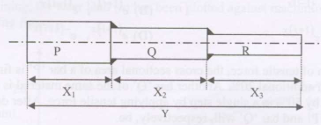
\includegraphics[width=0.5\linewidth]{figures/gate-pi-2008-40.png}
       \label{fig:q40}
   \end{figure}
   
\begin{tabularx}{\linewidth}{|X|X|X|}
\hline
Component & Mean Length (mm) & Tolerance (mm) \\
\hline 
P & $X_1=18$   & $\pm1.2$   \\
\hline
Q & $X_2=23$  & $\pm1.0$ \\
\hline
R & $X_3=24$ & $\pm1.5$\\
\hline
\end{tabularx}
    \begin{multicols}{4}
    \begin{enumerate}
        \item $65\pm2.16$
        \item $65\pm1.16$
        \item $65\pm6.16$
        \item $65\pm0.16$
    \end{enumerate}
\end{multicols}
\vspace{1cm}
 \item %Q.41}] 
 For the partial differential equation $\frac{\partial^2u}{\partial x^2}=\pi^2\frac{\partial u}{\partial t }$ in the domain $0\leq x\leq 1$ with boundary conditions $u(0,t)=0$ and $u(1,t)=0$ and initial condition $u(x,0)=\sin (\pi x)$, the solution of the differntial equation is 
    \hfill{(PI 2008)}
    \begin{multicols}{4}
    \begin{enumerate}
        \item $e^{-t}\sin (\pi x)$
        \item $e^{t}\sin (\pi x)$
        \item $e^{\pi t}\sin (\pi x)$
        \item $e^{-\pi t}\sin (\pi x)$
    \end{enumerate}
\end{multicols}
\vspace{1cm}
 \item %Q.42}]
 Inverse of the matrix 
 \myvec{
 0 & 1 & 0 \\
 1 & 0 & 0 \\
 0 & 0 & 1 }

    \hfill{(PI 2008)}
    \begin{multicols}{4}
    \begin{enumerate}
        \item $\myvec
           { 0 & 1 & 0 \\
            1 & 0 & 0 \\
            0 & 0 & 1} $
        
        \item $\myvec{
            0 & 1 & 0 \\
            1 & 0 & 0 \\
            0 & 0 & 1} 
        $
        \item $\myvec
            {0 & 1 & 0 \\
            1 & 0 & 0 \\
            0 & 0 & 1} 
        $
        \item $\myvec
           { 0 & 1 & 0 \\
            1 & 0 & 0 \\
            0 & 0 & 1} 
        $
    \end{enumerate}
\end{multicols}
\vspace{1cm}

 \item %Q.43}]
 For real x, the maximum value of $\frac{e^{\sin (x)}}{e^{\cos}(x)}$
    \hfill{(PI 2008)}
    \begin{multicols}{4}
    \begin{enumerate}
        \item $1$
        \item $e$
        \item $e^{\sqrt{2}}$
        \item $e^{\frac{1}{\sqrt 2}}$
    \end{enumerate}
\end{multicols}
\vspace{1cm}
 \item %Q.44}]
 A 19-tooth pinion paired with a 33-tooth gear has a 2-mm module and 20 degree pressure angle. Tooth forms are standard AGMA full depth involutes. If the center distance, during assembly, is increased by 3 percent, then the new pressure angle (in degrees) will be   
    \hfill{(PI 2008)}
    \begin{multicols}{4}
    \begin{enumerate}
        \item 
    $24.17$
        \item $22.21$
        \item $17.49$
        \item $34.45$
        \item $38.76$
    \end{enumerate}
\end{multicols}
\vspace{1cm}

\item %Q.45}]
The solutions of the differential equation 
\[
\frac{d^{2}y}{dx^{2}} + 2 \frac{dy}{dx} + 2y = 0
\]
are  
\hfill{(PI 2008)}
\begin{multicols}{4}
    \begin{enumerate}
\item[a] $e^{-(1+i)x},\ e^{-(1-i)x}$
\item[b)] $e^{(1+i)x},\ e^{(1-i)x}$
\item[c)] $e^{-(1+i)x},\ e^{(1+i)x}$
\item[d)] $e^{(1+i)x},\ e^{-(1+i)x}$
\end{enumerate}
    \end{multicols}
\vspace{1cm}

\item %mQ.46}]
By application of tensile force, the cross sectional area of a bar `P' is first reduced by 30\% and then by an additional 20\%. Another bar `Q' of the same material is reduced in cross sectional area by 50\% in a single step by applying tensile force. After deformation, the true strains in bar `P' and bar `Q' will, respectively, be  \hfill{(PI 2008)}
\begin{multicols}{4}
    \begin{enumerate}
\item[a)] 0.50 and 0.50
\item[b)] 0.58 and 0.69
\item[c)] 0.69 and 0.69
\item[d)] 0.78 and 1.00
\end{enumerate}
    \end{multicols}
\vspace{1cm}

\item %Q.47}]
In sand casting of a hollow part of lead, a cylindrical core of diameter 120 mm and height 180 mm is placed inside the mould cavity. The densities of core material and lead are 1600 $\mathrm{kg/m^3}$ and 11300 $\mathrm{kg/m^3}$ respectively. The net force (in N) that tends to lift the core during pouring of molten metal will be  \hfill{(PI 2008)}
\begin{multicols}{4}
    \begin{enumerate}
\item[a)] 19.7
\item[b)] 64.5
\item[c)] 193.7
\item[d)] 257.6
\end{enumerate}
\end{multicols}
\vspace{1cm}

\item %Q.48}]
Aluminium strips of 2 mm thickness are joined together by resistance spot welding process by applying an electric current of 6000 A for 0.15 sec. The heat required for melting aluminium is$2.9J/m^3$. The diameter and the thickness of weld nugget are found to be 5 mm and 2.5 mm, respectively. Assuming the electrical resistance to be 75 $\mu\Omega$, the percentage of total energy utilized in forming the weld nugget is:\hfill{(PI 2008)}
\begin{multicols}{4}
    \begin{enumerate}
  \item[a)] 28
  \item[b)] 35
  \item[c)] 65
  \item[d)] 72
\end{enumerate}
\end{multicols}
\vspace{1cm}
\item %Q.49}]
In a rolling process, thickness of a strip is reduced from 4 mm to 3 mm using 300 mm diameter rolls rotating at 100 rpm. The velocity of the strip (in m/sec) at the neutral point is:\hfill{(PI 2008)}
\begin{multicols}{4}
    \begin{enumerate}
  \item[a)] 1.57
  \item[b)] 3.14
  \item[c)] 47.10
  \item[d)] 94.20
\end{enumerate}
\end{multicols}
\vspace{1cm}

\item %Q.50}]
A blank of 50 mm diameter is to be sheared from a sheet of 2.5 mm thickness. The required radial clearance between the die and the punch is 6\% of sheet thickness. The punch and die diameters (in mm) for this blanking operation, respectively, are:\hfill{(PI 2008)}
\begin{multicols}{4}
    \begin{enumerate}
  \item[a)] 50.00 and 50.30
  \item[b)] 50.00 and 50.15
  \item[c)] 49.70 and 50.00
  \item[d)] 49.85 and 50.00
\end{enumerate}
\end{multicols}
\vspace{1cm}

\item %Q.51}]
In an electrochemical machining (ECM) operation, a square hole of dimensions 5 mm $\times$ 5 mm is drilled in a block of copper. The current used is 5000 A. Atomic weight of copper is 63 and valency of dissolution is 1. Faraday's constant is 96500 Coulomb. The material removal rate (in g/s) is:\hfill{(PI 2008)}
\begin{multicols}{4}
    \begin{enumerate}
  \item[a)] 0.326
  \item[b)] 3.260
  \item[c)] \( 3.15 \times 10^3 \)
  \item[d)] \( 3.15 \times 10^5 \)
\end{enumerate}
\end{multicols}
\vspace{1cm}

\item %Q.52}]
A shaft of diameter 10 mm transmits 100 W of power at an angular speed of \( \frac{800}{\pi} \) rad/s. The maximum shear stress (in MPa) developed in the shaft is:\hfill{(PI 2008)}
\begin{multicols}{4}
    \begin{enumerate}
  \item[a)] 2
  \item[b)] 4
  \item[c)] 8
  \item[d)] 16
\end{enumerate}
\end{multicols}
\vspace{1cm}
\item %Q.53}]
During machining, the wear land $(h)$ has been plotted against machining time $(T)$ as given in the following figure. \\[2mm]

\begin{figure}[h]
    \centering
    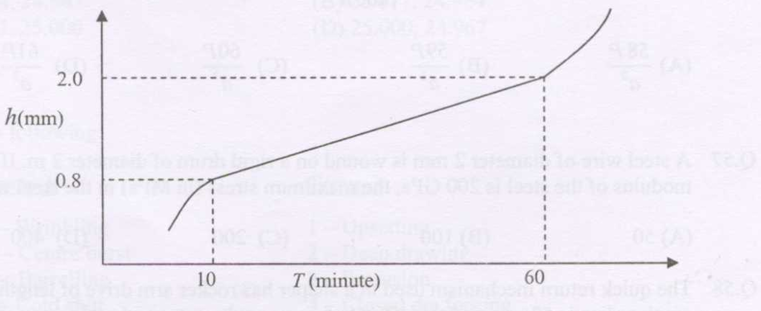
\includegraphics[width=0.5\linewidth]{figures/GATE-pi-2008-51.png}
    \caption{Caption}
    \label{q53}
\end{figure}

For a critical wear land of $1.8 \ \mathrm{mm}$, the cutting tool life (in minute) is  \hfill{(PI 2008)}
\begin{multicols}{4}
    \begin{enumerate}
\item[a)] 52.00
\item[b)] 51.67
\item[c)] 51.50
\item[d)] 50.00
\end{enumerate}
\end{multicols}
\vspace{1cm}
\item %Q.54}] 
A strain rosette, as shown in the figure, has three strain gauges P, Q and R.  



If the values of strain indicated in the three strain gauges are  
\[
\varepsilon_P = 100 \times 10^{-6}, \quad
\varepsilon_Q = 150 \times 10^{-6}, \quad
\varepsilon_R = 200 \times 10^{-6}
\]
the largest principal strain is  \hfill{(PI 2008)}
\begin{multicols}{4}
    \begin{enumerate}
\item[a)] $200 \times 10^{-6}$
\item[b)] $250 \times 10^{-6}$
\item[c)] $300 \times 10^{-6}$
\item[d)] $350 \times 10^{-6}$
\end{enumerate}
\end{multicols}
\vspace{1cm}

\item %Q.55}] 
A cantilever beam XY of length 2 m and cross-sectional dimensions $25\ \mathrm{mm} \times 25\ \mathrm{mm}$ is fixed at X and is subjected to a moment of $100\ \mathrm{N \cdot m}$ and an unknown force P at the free end Y as shown in the figure. The Young's modulus of the material of the beam is $200\ \mathrm{GPa}$.  

\begin{figure}[h]
    \centering
    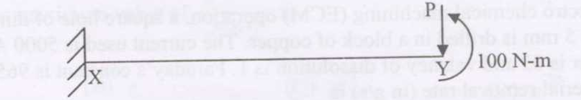
\includegraphics[width=0.5\linewidth]{figures/GATE-pi-2008-55.png}
    \caption{Caption}
    \label{q55}
\end{figure}

If the deflection of the free end Y is zero, then the value of P (in N) is  \hfill{(PI 2008)}
\begin{multicols}{4}
    \begin{enumerate}
\item[a)] 67
\item[b)] 75
\item[c)] 133
\item[d)] 150
\end{enumerate}
\end{multicols}
\vspace{1cm}


\item %Q.56}] 
A frame of square cross-section of $(a \times a)$ is as shown in the figure. The stress near the fixed end on the upper side of the frame is  \hfill{(PI 2008)}

\begin{figure}[h]
    \centering
    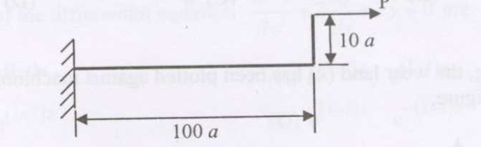
\includegraphics[width=0.5\linewidth]{figures/GATE-pi-2008-56.png}
    \caption{Caption}
    \label{q56}
\end{figure}

\begin{multicols}{4}
    \begin{enumerate}
\item[a)] $\dfrac{58P}{a^2}$
\item[b)] $\dfrac{59P}{a^2}$
\item[c)] $\dfrac{60P}{a^2}$
\item[d)] $\dfrac{61P}{a^2}$
\end{enumerate}
\end{multicols}
\vspace{1cm}
\item %Q.57}]
\hfill{(PI 2008)}
\begin{multicols}{4}
    \begin{enumerate}
\item[a)] 50
\item[b)] 100
\item[c)] 200
\item[d)] 400
\end{enumerate}
\end{multicols}
\vspace{1cm}

\item %Q.58}] 
The quick return mechanism used in a shaper has rocker arm drive of length 200 mm. If the crank radius is 50 mm and the offset between crank centre and rocker arm pivot is 20 mm, length of the stroke (in m) is  \hfill{(PI 2008)}
\begin{multicols}{4}
    \begin{enumerate}
\item[a)] 0.5
\item[b)] 1.0
\item[c)] 1.5
\item[d)] 2.0
\end{enumerate}
\end{multicols}
\vspace{1cm}
\item %Q.59}]
A stepper motor has 150 steps. The output shaft of the motor is directly coupled to a lead screw of pitch 4 mm, which drives a table. If the frequency of pulse supply to the motor is 200 Hz, the speed of the table (in mm/min) is  \hfill{(PI 2008)}
\begin{multicols}{4}
    \begin{enumerate}
\item[a)] 400
\item[b)] 320
\item[c)] 300
\item[d)] 280
\end{enumerate}
\end{multicols}
\vspace{1cm}


\item %Q.60}]
An experimental setup is planned to determine the taper of workpiece as shown in the figure. If the two precision rollers have radii 8 mm and 5 mm and the total thickness of slip gauges inserted between the rollers is 15.54 mm, the taper angle $\theta$ is:\hfill{(PI 2008)}

\begin{figure}
    \centering
    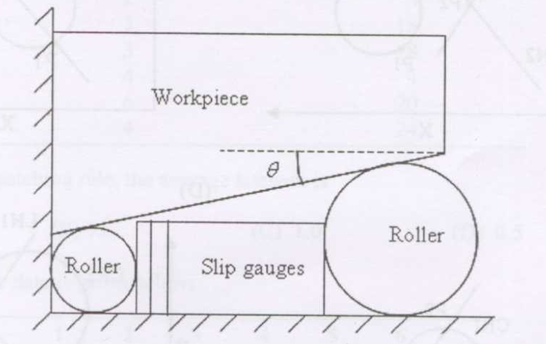
\includegraphics[width=0.5\linewidth]{figures/GATE-pi-2008-60.png}
    \caption{Caption}
    \label{q60}
\end{figure}
\begin{multicols}{4}
    \begin{enumerate}
\item 6 degree 
b) 10 degree 
c) 11 degree
d) 12 degree

\end{enumerate}
\end{multicols}
\vspace{1cm}
\item %Q.61}]
Following data are given for calculating limits of dimensions and tolerances for a hole:  
Tolerance unit $i$ ($\mu m$) $= 0.45\sqrt[3]{D} + 0.001D$.  
The unit of $D$ is mm. Diameter step is 18--30 mm.  
If the fundamental deviation for H hole is zero and $IT8 = 25i$, the maximum and minimum limits of dimension for a 25 mm H8 hole (in mm) are:\hfill{(PI 2008)}

\begin{multicols}{4}
    \begin{enumerate}
\item  24.984, 24.967 
\item  25.017, 24.984 
\item  25.033, 25.000 
\item 25.000, 24.967

\end{enumerate}
\end{multicols}


\vspace{0.5cm}
\item %Q.62}] 
Match the following:  
\hfill{(PI 2008)}\\
\begin{tabular}{ll}
\textbf{Group 1} & \textbf{Group 2} \\
P -- Wrinkling & 1 -- Upsetting \\
Q -- Centre burst & 2 -- Deep drawing \\
R -- Barrelling & 3 -- Extrusion \\
S -- Cold shut & 4 -- Closed die forging \\
\end{tabular}

\begin{multicols}{4}
    \begin{enumerate}
\item  P-2, Q-3, R-4, S-1 
\item  P-3, Q-4, R-1, S-2 
\item  P-2, Q-3, R-1, S-4 
\item  P-2, Q-4, R-3, S-1
\end{enumerate}
\end{multicols}
\vspace{1cm}

\item %Q.63}] 
Suppose point $P_1$ in APT (Automatically Programmed Tool) programming is coded by statement  
\[
P_1 = \text{POINT/ XSMALL, INTOF, LN1, CR1}
\]  
The coded geometric situation without causing error is:
\hfill{(PI 2008)}
\begin{itemize}

   

    \item[a)]\begin{figure}[h]
    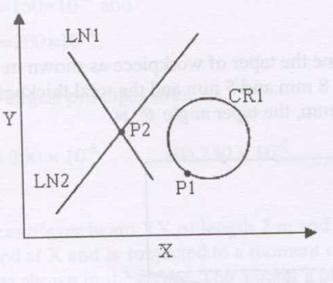
\includegraphics[width=0.35\textwidth]{figures/63-a-pi-2008-gate.png}
    \caption{}
    \label{q63a}
    \end{figure}
    \item[b)]\begin{figure}[h] 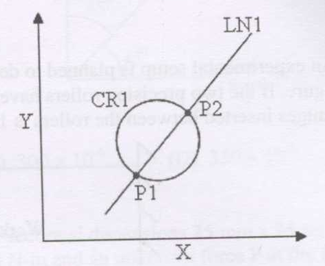
\includegraphics[width=0.35\textwidth]{figures/63-b-pi-2008-gate.png}
    \caption{}
    \label{q63b}
    \end{figure}
    \item[c)]\begin{figure}[h] 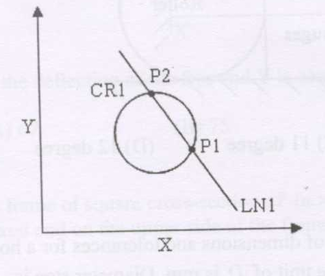
\includegraphics[width=0.35\textwidth]{figures/63-c-pi-2008-gate.png}
    \caption{}
    \label{q63c}
    \end{figure}
    \item[d)]\begin{figure}[h] 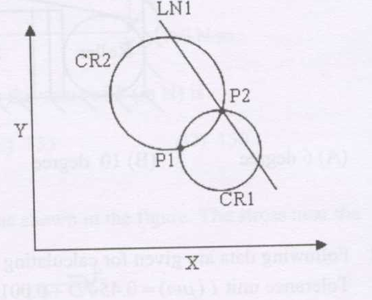
\includegraphics[width=0.35\textwidth]{figures/63-d-pi-2008-gate.png}
    \caption{}
    \label{q63d}
    \end{figure}
\end{itemize}


\vspace{0.5cm}
\item %Q.64}] 
Match the following:
\hfill{(PI 2008)}\\
\begin{tabular}{ll}
\textbf{Group 1} & \textbf{Group 2} \\
P -- Mulling & 1 -- Powder metallurgy \\
Q -- Impregnation & 2 -- Injection moulding \\
R -- Flash trimming & 3 -- Processing of FRP composites \\
S -- Curing & 4 -- Sand casting \\
\end{tabular}

\noindent
a) P-4, Q-3, R-2, S-1 \\
b) P-2, Q-4, R-3, S-1 \\
c) P-2, Q-1, R-4, S-3 \\
d) P-4, Q-1, R-2, S-3

\vspace{0.5cm}
\item %Q.65}]
When P is the rate of production, D is the demand rate and l is the duration production, the actual inventory built up during production period in the EPQ model is 
\hfill{(PI 2008)}
\begin{multicols}{4}
    \begin{enumerate}
\item Zero
\item $(P+D)t$
\item $Pt$
\item $\frac{(P-D)}{t}$
    
    \end{enumerate}
\end{multicols}
\vspace{1cm}

\item %Q.66}]
Consider the following work sampling data:  
Working time = 60\%, average rating = 90\%, relaxation allowance = 12.5\%,  
actual output during the study = 1000 units and study duration = 480 minutes.  
The standard time per unit (in minutes) will be:
\hfill{(PI 2008)}

\begin{multicols}{4}
    \begin{enumerate}
\item  0.2592
\item  0.2916
\item  0.3240 
\item  0.4860
 \end{enumerate}
\end{multicols}
\vspace{1cm}
\vspace{0.5cm}
\item %Q.67}]
Six jobs are received for processing and their processing times and delivery dates are given below:
\hfill{(PI 2008)}
\begin{center}
\begin{tabular}{|c|c|c|}
\hline
\textbf{Job Sequence} & \textbf{Production Time (days)} & \textbf{Delivery Date (days)} \\
\hline
P & 2 & 4 \\
Q & 5 & 18 \\
R & 3 & 8 \\
S & 7 & 4 \\
T & 6 & 20 \\
U & 4 & 24 \\
\hline
\end{tabular}
\end{center}

Using FCFS dispatching rule, the average lateness is:  

\begin{multicols}{4}
    \begin{enumerate}
\item 2.0 
\item1.5 
\item1.0 
\item0.5
 \end{enumerate}
\end{multicols}
\vspace{1cm}
\vspace{0.5cm}
\item %Q.68}]
An assembly line data is given below:
\hfill{(PI 2008)}
\begin{center}
\begin{tabular}{|c|c|c|c|c|c|c|}
\hline
\textbf{Station} & 1 & 2 & 3 & 4 & 5 & 6 \\
\hline
Cycle time & 90 & 90 & 90 & 90 & 90 & 90 \\
Task time  & 70 & 70 & 80 & 70 & 80 & 60 \\
Idle time  & 20 & 20 & 10 & 20 & 10 & 30 \\
\hline
\end{tabular}
\end{center}

The percentage utilization of labour on the assembly line is:  

\begin{multicols}{4}
    \begin{enumerate}
\item a) 20.37
\item b) 25.58 
\item c) 26.63  
\item d) 79.62
 \end{enumerate}
\end{multicols}
\vspace{1cm}
\item %Q.69}]
In mostly accepted and applicable PTS systems (i.e. MTM-2), the motions and their codes are specified. Match the following:
\hfill{(PI 2008)}\\
\vspace{1cm}
\begin{tabular}{ll}
\textbf{Group 1} & \textbf{Group 2} \\
P -- Weight factors & 1 -- GW \\
Q -- GET            & 2 -- GA \\
R -- PUT            & 3 -- PB \\
S -- Apply pressure & 4 -- A \\
\end{tabular}

\begin{multicols}{4}
    \begin{enumerate}
\item  P-1, Q-3, R-4, S-2 
\item P-2, Q-1, R-3, S-4 
\item P-1, Q-4, R-3, S-2 
\item P-1, Q-2, R-3, S-4

 \end{enumerate}
\end{multicols}
\vspace{1cm}
\item %Q.70}]
Daily demand of a product is normally distributed with a mean of 50 units and a standard deviation of 5. Supply conditions are virtually certain with a lead time of 6 days. If a 95\% percent service level is desired, the reorder point ($z_{0.95} = 1.645$) is:
\hfill{(PI 2008)}
\begin{multicols}{4}
    \begin{enumerate}
\item  340 units 
\item  320 units 
\item  300 units
\item  280 units

 \end{enumerate}
\end{multicols}
\vspace{1cm}

\textbf{Common Data Questions}\\
\textbf{Common Data for Questions 71, 72 and 73:}  

The figure illustrates a PERT network describing the precedence relationship among different activities.  
The optimistic time, most likely time and pessimistic time of the activities are given in the table below.

\begin{figure}
    \centering
    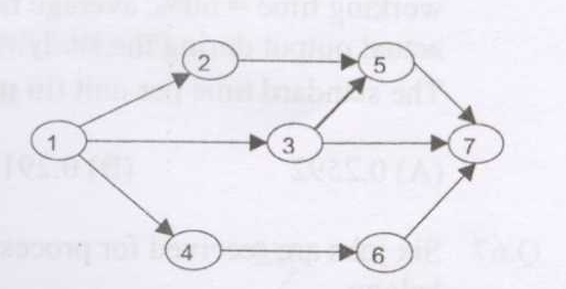
\includegraphics[width=0.5\linewidth]{figures/71-73-pi-2008-gate.png}
    \caption{}
    \label{q71}
\end{figure}

\begin{center}
\begin{tabular}{|c|c|c|c|}
\hline
\textbf{Activity} & \textbf{Optimistic time (hour)} & \textbf{Most likely time (hour)} & \textbf{Pessimistic time (hour)} \\
\hline
1-2 & 7 & 9 & 11 \\
1-3 & 5 & 7 & 9 \\
1-4 & 4 & 7 & 12 \\
2-5 & 8 & 10 & 12 \\
3-5 & 8 & 10 & 12 \\
3-6 & 7 & 10 & 12 \\
4-6 & 4 & 8 & 12 \\
5-7 & 5 & 8 & 11 \\
6-7 & 3 & 5 & 7 \\
\hline
\end{tabular}
\end{center}

\noindent
\item %Q.71}]
The length of the critical path (in hours) is: \hfill{(PI 2008)}
\begin{multicols}{4}
    \begin{enumerate}
\item  17 
\item 18 
\item 24 
\item 27
\end{enumerate}
\end{multicols}
\vspace{1cm}
\vspace{0.4cm}

\item %Q.72}]
The standard deviation of the critical path (in hours) is:\hfill{(PI 2008)}  
\begin{multicols}{4}
    \begin{enumerate}
\item 0.66 
\item 0.94 
\item 1.37 
\item 1.56
 \end{enumerate}
\end{multicols}
\vspace{1cm}
\noindent
\item %Q.73}]
The slack at event number 3 (in hours) is: \hfill{(PI 2008)}
\begin{multicols}{4}
    \begin{enumerate}
\item 0 
\item 3
\item 6 
\item 10

 \end{enumerate}
\end{multicols}
\vspace{1cm}
\textbf{Common Data for Questions 74 and 75:}  

A quadratic Bezier curve segment is described by  
\[
\vec{r}(u) = \sum_{i=0}^{2} B_{i,2} \vec{r}_i
\]
where $\vec{r}_i$ and $B_{i,2}$ are control points and blending functions respectively.  
Given:  
\[
B_{i,2} = \binom{2}{i} u^i (1-u)^{2-i}, \quad u \in [0,1]
\]
Consider $(0,0)$, $(4,4)$ and $(12,8)$ as the control points of the Bezier curve.

\vspace{0.4cm}
\noindent
\item %Q.74}]
The point $(1,2)$ lies:  \hfill{(PI 2008)}

a on the Bezier curve \\
b) on the boundary of the convex hull \\
c) outside the convex hull \\
d) within the convex hull but not on the Bezier curve \\

\vspace{1cm}
\noindent
\item %Q.75}]
Slope of the tangent at point $(5,4)$ to the Bezier curve is: \hfill{(PI 2008)}
\begin{multicols}{4}
    \begin{enumerate}
\item  $-0.667$ 
\item $-0.333$ 
\item $0.333$
\item $0.667$

 \end{enumerate}
\end{multicols}
\vspace{1cm}

\textbf{Statement for Linked Answer Questions 76 and 77:}

A wall is heated uniformly at a volumetric heat generation rate of 1 kW/m$^3$.  
The temperature distribution across the 1 m thick wall at a certain instant of time is given by:  
\[
T(x) = a + b x + c x^2
\]
where $a = 900^\circ \text{C}$, $b = -300^\circ \text{C/m}$, and $c = -50^\circ \text{C/m}^2$.  

The wall has an area of 10 m$^2$ (as shown in the figure) and a thermal conductivity of 40 W/mK.

\begin{figure}
    \centering
    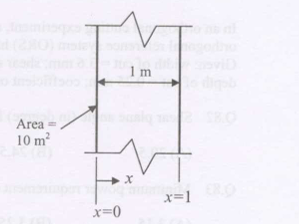
\includegraphics[width=0.5\linewidth]{figures/76-77-pi-2008-gate.png}
    \caption{}
    \label{q76}
\end{figure}
\noindent
\item %Q.76}] 
The rate of heat transfer (in kW) into the wall (at $x=0$) is:\hfill{(PI 2008)}
\begin{multicols}{4}
    \begin{enumerate}
\item 900 
\item 450  
\item 120  
\item 60

 \end{enumerate}
\end{multicols}
\vspace{1cm}

\noindent
\item %Q.77}]
The rate of change of energy storage (in kW) in the wall is:\hfill{(PI 2008)}
\begin{multicols}{4}
    \begin{enumerate}
\item  130 
\item 120 
\item $-10$
\item $-30$

 \end{enumerate}
\end{multicols}
\vspace{1cm}

\section*{Statement for Linked Answer Questions 78 and 79:}

A disk brake has two friction linings with the outside-lining and inside-lining diameters as 120 mm and 60 mm, respectively.  
The coefficient of friction at the interface of lining and rotating part is 0.35.  
A 10 kN axial force is applied to stop the part rotating at 8000 rpm.  
To cool the disk brake, an arrangement of circulating the water (specific heat 4.2 kJ/kg$^\circ$C) is made.  
Assume uniform wear rate of disk linings and heat transfer by convection only.


\textbf{Q.78} The torque (in N·m) applied by the brake on the rotating part is:\hfill{(PI 2008)} 
\begin{multicols}{4}
    \begin{enumerate}
\item  215  
\item 315 
\item 630 
\item 1260

 \end{enumerate}
\end{multicols}
\vspace{1cm}


\item %Q.79}]
temperature rise of $3^\circ$C is:
\hfill{(PI 2008)}
\begin{multicols}{4}
    \begin{enumerate}
\item  2.2 
\item 3.4  
\item 10.4  
\item 21.0

 \end{enumerate}
\end{multicols}
\vspace{1cm}

\textbf{Statement for Linked Answer Questions 80 and 81:}

A 10 mm diameter annealed steel wire is drawn through a die at a speed of 0.5 m/s to reduce the diameter by 20\%.  
The yield stress of the material is 800 MPa.

\noindent
\item %Q.80}]
Neglecting friction and strain hardening, the stress required for drawing (in MPa) is: \hfill{(PI 2008)}
\begin{multicols}{4}
    \begin{enumerate}
\item  178.5 
\item 357.0 
\item 1287.5 
\item 2575.0

 \end{enumerate}
\end{multicols}
\vspace{1cm}

\noindent
\item %Q.81}]
The power required for the drawing process (in kW) is: \hfill{(PI 2008)}
\begin{multicols}{4}
    \begin{enumerate}
\item  8.97
\item 14.0 
\item 17.95 
\item 28.0
 \end{enumerate}
\end{multicols}
\vspace{1cm}

\textbf{Statement for Linked Answer Questions 82 and 83:}

In an orthogonal cutting experiment, an HSS tool having the following tool signature in the orthogonal reference system (ORS) has been used: 0-10-7-7-10-75-1.  

Given: width of cut = 3.6 mm; shear strength of workpiece material = 460 N/mm$^2$;  
depth of cut = 0.25 mm; coefficient of friction at tool-chip interface = 0.7.  


    \item %Q.82}] 
    Shear plane angle (in degree) for minimum cutting force is \hfill{(PI 2008)} 
    \begin{enumerate}
        \item 20.5
        \item 24.5
        \item 28.5
        \item 32.5
    \end{enumerate}

    \item %Q.83}]
    Minimum power requirement (in kW) at a cutting speed of 150 m/min is  \hfill{(PI 2008)}
    \begin{enumerate}
        \item 3.15
        \item 3.25
        \item 3.35
        \item 3.45
    \end{enumerate}


\textbf{Statement for Linked Answer Questions 84 and 85:}

A company forecasts the demand for a product to be 400 units per month for each of the next three months. The actual demand, however, turned out to be 400, 550 and 580 units respectively for those three months.


    \item %Q.84}]
    The forecast error bias is \hfill{(PI 2008)} 
    \begin{enumerate}
        \item -330 units
        \item -110 units
        \item 110 units
        \item 330 units
    \end{enumerate}

    \item %Q.85}]
    The forecasting technique used has a tendency to \hfill{(PI 2008)} 
    \begin{enumerate}
        \item under forecast with 21.56\% bias
        \item over forecast with 21.56\% bias
        \item under forecast with 64.70\% bias
        \item over forecast with 64.70\% bias
    \end{enumerate}
\vspace{6cm}
{END OF THE QUESTION PAPER}


























    




    
    \end{enumerate}
\end{document}